% Options for packages loaded elsewhere
\PassOptionsToPackage{unicode}{hyperref}
\PassOptionsToPackage{hyphens}{url}
\PassOptionsToPackage{dvipsnames,svgnames*,x11names*}{xcolor}
%
\documentclass[
  english,
  man,floatsintext]{apa6}
\usepackage{lmodern}
\usepackage{amssymb,amsmath}
\usepackage{ifxetex,ifluatex}
\ifnum 0\ifxetex 1\fi\ifluatex 1\fi=0 % if pdftex
  \usepackage[T1]{fontenc}
  \usepackage[utf8]{inputenc}
  \usepackage{textcomp} % provide euro and other symbols
\else % if luatex or xetex
  \usepackage{unicode-math}
  \defaultfontfeatures{Scale=MatchLowercase}
  \defaultfontfeatures[\rmfamily]{Ligatures=TeX,Scale=1}
\fi
% Use upquote if available, for straight quotes in verbatim environments
\IfFileExists{upquote.sty}{\usepackage{upquote}}{}
\IfFileExists{microtype.sty}{% use microtype if available
  \usepackage[]{microtype}
  \UseMicrotypeSet[protrusion]{basicmath} % disable protrusion for tt fonts
}{}
\makeatletter
\@ifundefined{KOMAClassName}{% if non-KOMA class
  \IfFileExists{parskip.sty}{%
    \usepackage{parskip}
  }{% else
    \setlength{\parindent}{0pt}
    \setlength{\parskip}{6pt plus 2pt minus 1pt}}
}{% if KOMA class
  \KOMAoptions{parskip=half}}
\makeatother
\usepackage{xcolor}
\IfFileExists{xurl.sty}{\usepackage{xurl}}{} % add URL line breaks if available
\IfFileExists{bookmark.sty}{\usepackage{bookmark}}{\usepackage{hyperref}}
\hypersetup{
  pdftitle={Epidemiologische situatie COVID-19 in Nederland - 02 november 2021},
  pdfauthor={Marino van Zelst1},
  pdflang={en-EN},
  colorlinks=true,
  linkcolor=Maroon,
  filecolor=Maroon,
  citecolor=Blue,
  urlcolor=blue,
  pdfcreator={LaTeX via pandoc}}
\urlstyle{same} % disable monospaced font for URLs
\usepackage{graphicx,grffile}
\makeatletter
\def\maxwidth{\ifdim\Gin@nat@width>\linewidth\linewidth\else\Gin@nat@width\fi}
\def\maxheight{\ifdim\Gin@nat@height>\textheight\textheight\else\Gin@nat@height\fi}
\makeatother
% Scale images if necessary, so that they will not overflow the page
% margins by default, and it is still possible to overwrite the defaults
% using explicit options in \includegraphics[width, height, ...]{}
\setkeys{Gin}{width=\maxwidth,height=\maxheight,keepaspectratio}
% Set default figure placement to htbp
\makeatletter
\def\fps@figure{htbp}
\makeatother
\setlength{\emergencystretch}{3em} % prevent overfull lines
\providecommand{\tightlist}{%
  \setlength{\itemsep}{0pt}\setlength{\parskip}{0pt}}
\setcounter{secnumdepth}{-\maxdimen} % remove section numbering
% Make \paragraph and \subparagraph free-standing
\ifx\paragraph\undefined\else
  \let\oldparagraph\paragraph
  \renewcommand{\paragraph}[1]{\oldparagraph{#1}\mbox{}}
\fi
\ifx\subparagraph\undefined\else
  \let\oldsubparagraph\subparagraph
  \renewcommand{\subparagraph}[1]{\oldsubparagraph{#1}\mbox{}}
\fi
% Manuscript styling
\usepackage{upgreek}
\captionsetup{font=singlespacing,justification=justified}

% Table formatting
\usepackage{longtable}
\usepackage{lscape}
% \usepackage[counterclockwise]{rotating}   % Landscape page setup for large tables
\usepackage{multirow}		% Table styling
\usepackage{tabularx}		% Control Column width
\usepackage[flushleft]{threeparttable}	% Allows for three part tables with a specified notes section
\usepackage{threeparttablex}            % Lets threeparttable work with longtable

% Create new environments so endfloat can handle them
% \newenvironment{ltable}
%   {\begin{landscape}\begin{center}\begin{threeparttable}}
%   {\end{threeparttable}\end{center}\end{landscape}}
\newenvironment{lltable}{\begin{landscape}\begin{center}\begin{ThreePartTable}}{\end{ThreePartTable}\end{center}\end{landscape}}

% Enables adjusting longtable caption width to table width
% Solution found at http://golatex.de/longtable-mit-caption-so-breit-wie-die-tabelle-t15767.html
\makeatletter
\newcommand\LastLTentrywidth{1em}
\newlength\longtablewidth
\setlength{\longtablewidth}{1in}
\newcommand{\getlongtablewidth}{\begingroup \ifcsname LT@\roman{LT@tables}\endcsname \global\longtablewidth=0pt \renewcommand{\LT@entry}[2]{\global\advance\longtablewidth by ##2\relax\gdef\LastLTentrywidth{##2}}\@nameuse{LT@\roman{LT@tables}} \fi \endgroup}

% \setlength{\parindent}{0.5in}
% \setlength{\parskip}{0pt plus 0pt minus 0pt}

% \usepackage{etoolbox}
\makeatletter
\patchcmd{\HyOrg@maketitle}
  {\section{\normalfont\normalsize\abstractname}}
  {\section*{\normalfont\normalsize\abstractname}}
  {}{\typeout{Failed to patch abstract.}}
\patchcmd{\HyOrg@maketitle}
  {\section{\protect\normalfont{\@title}}}
  {\section*{\protect\normalfont{\@title}}}
  {}{\typeout{Failed to patch title.}}
\makeatother
\shorttitle{Dagelijkse rapportage}
\DeclareDelayedFloatFlavor{ThreePartTable}{table}
\DeclareDelayedFloatFlavor{lltable}{table}
\DeclareDelayedFloatFlavor*{longtable}{table}
\makeatletter
\renewcommand{\efloat@iwrite}[1]{\immediate\expandafter\protected@write\csname efloat@post#1\endcsname{}}
\makeatother
\usepackage{csquotes}
\ifxetex
  % Load polyglossia as late as possible: uses bidi with RTL langages (e.g. Hebrew, Arabic)
  \usepackage{polyglossia}
  \setmainlanguage[]{english}
\else
  \usepackage[shorthands=off,main=english]{babel}
\fi

\title{Epidemiologische situatie COVID-19 in Nederland - 02 november 2021}
\author{Marino van Zelst\textsuperscript{1}}
\date{}


\affiliation{\vspace{0.5cm}\textsuperscript{1} Vragen over deze rapportage kunnen verstuurd worden aan Marino van Zelst, twitter.com/mzelst. E-mail: \href{mailto:j.m.vanzelst@uvt.nl}{\nolinkurl{j.m.vanzelst@uvt.nl}}}

\begin{document}
\maketitle

{
\hypersetup{linkcolor=}
\setcounter{tocdepth}{3}
\tableofcontents
}
\newpage

\hypertarget{samenvatting}{%
\section{Samenvatting}\label{samenvatting}}

\textbf{Samenvatting (op basis van GGD cijfers)}\\
Tot en met 2021-11-02 zijn er in Nederland in totaal 2147473 COVID-19 patiënten gemeld aan het RIVM. Tot nu toe zijn 33710 van de gemelde patiënten opgenomen in het ziekenhuis en 18441 mensen overleden.

\textbf{Gegevens t. o. v. gisteren}\\
Positief getest: 7761
Totaal: 2147473 (+ 7727 ivm -34 corr.)

Opgenomen: 36
Totaal: 33710 (+
35 ivm -1 corr.)

Overleden: 18
Totaal: 18441 (+
18 ivm 0 corr.)

\textbf{Update met betrekking tot ziekenhuis-gegevens (data NICE)}

Patiënten verpleegafdeling\\
Bevestigd: 15 Verdacht: 5

Patiënten IC\\
Bevestigd: 4 Verdacht: 1

\textbf{Data}\\
Een databestand met de cumulatieve aantallen per gemeente per dag van gemelde COVID-19 patiënten, in het ziekenhuis opgenomen COVID-19 patiënten en overleden COVID-19 patiënten is \href{https://data.rivm.nl/geonetwork/srv/dut/catalog.search\#/metadata/1c0fcd57-1102-4620-9cfa-441e93ea5604}{hier} te vinden. Een databestand met karakteristieken van elke positief geteste COVID-19 patiënt in Nederland is \href{https://data.rivm.nl/geonetwork/srv/dut/catalog.search\#/metadata/2c4357c8-76e4-4662-9574-1deb8a73f724?tab=relations}{hier} te vinden. Alle gegevens die voor dit rapport gebruikt worden zijn te vinden in de \href{https://github.com/mzelst/covid-19}{Github repository}.

\newpage

\hypertarget{covid-19-meldingen-in-de-afgelopen-vier-weken}{%
\section{COVID-19 meldingen in de afgelopen vier weken}\label{covid-19-meldingen-in-de-afgelopen-vier-weken}}

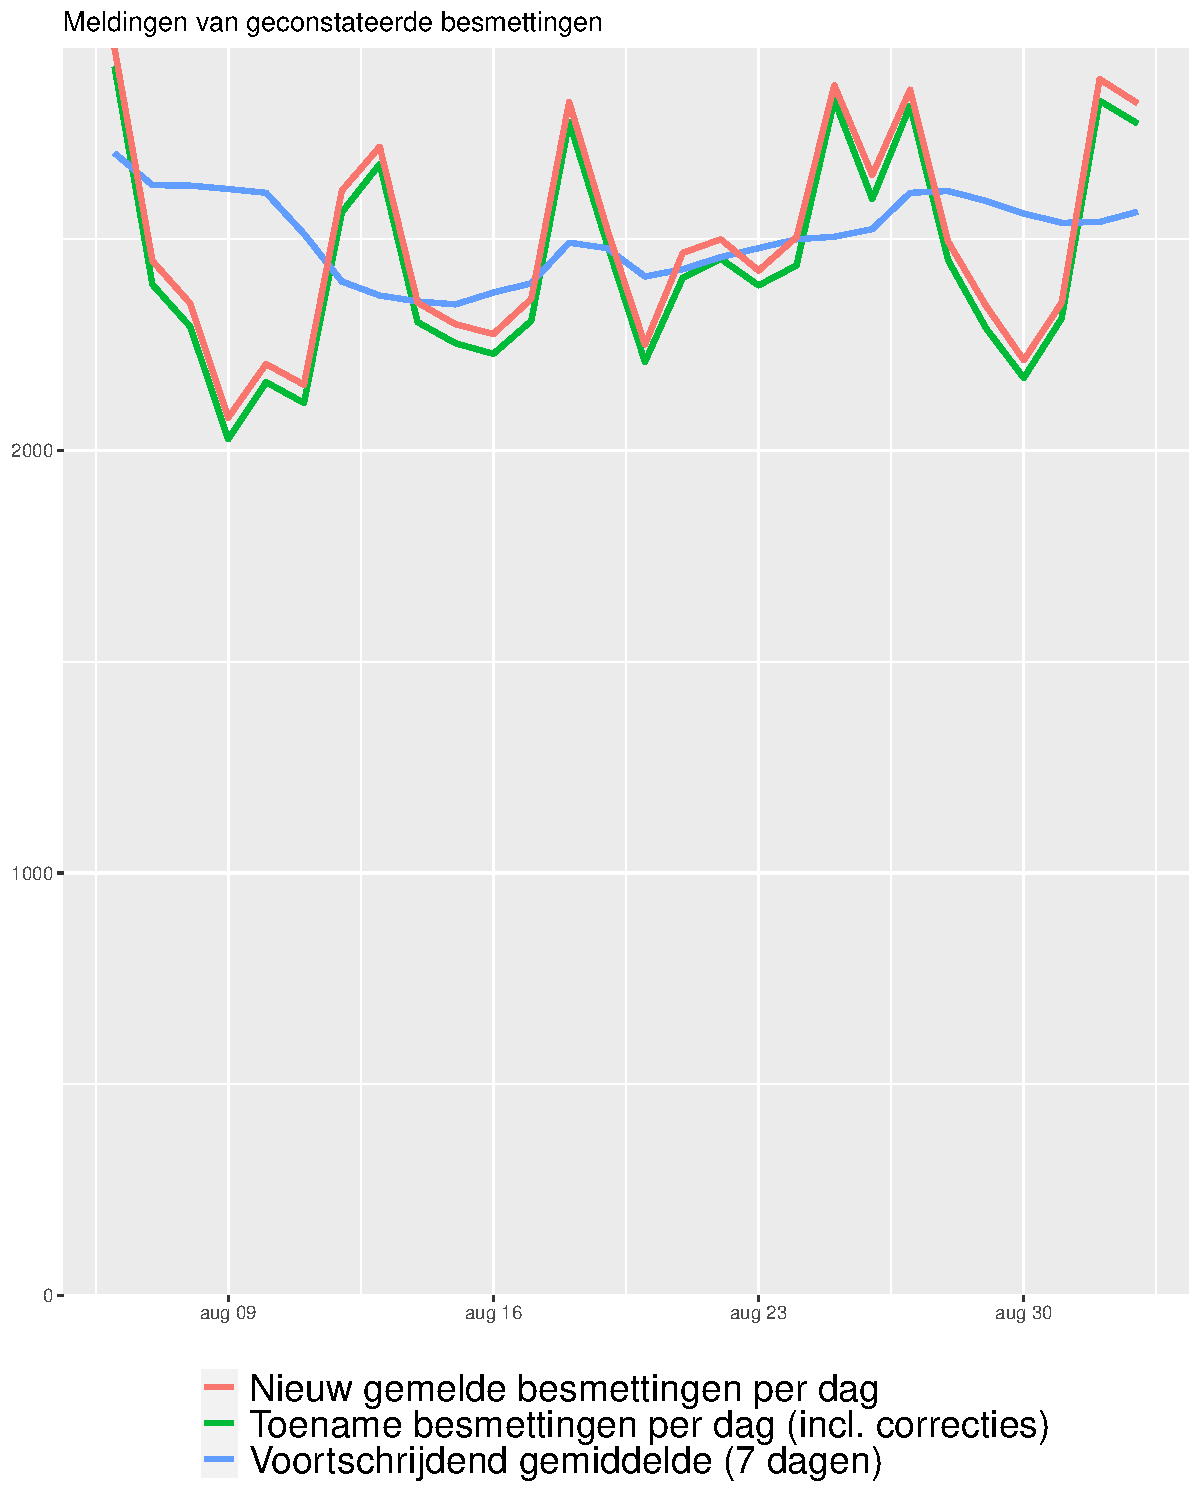
\includegraphics{daily_report_files/figure-latex/Gemelde besmettingen-1.pdf}

\newpage

\hypertarget{kaart-met-covid-19-meldingen-per-gemeente-sinds-gisteren}{%
\section{Kaart met COVID-19 meldingen per gemeente sinds gisteren}\label{kaart-met-covid-19-meldingen-per-gemeente-sinds-gisteren}}

\begin{figure}
\centering
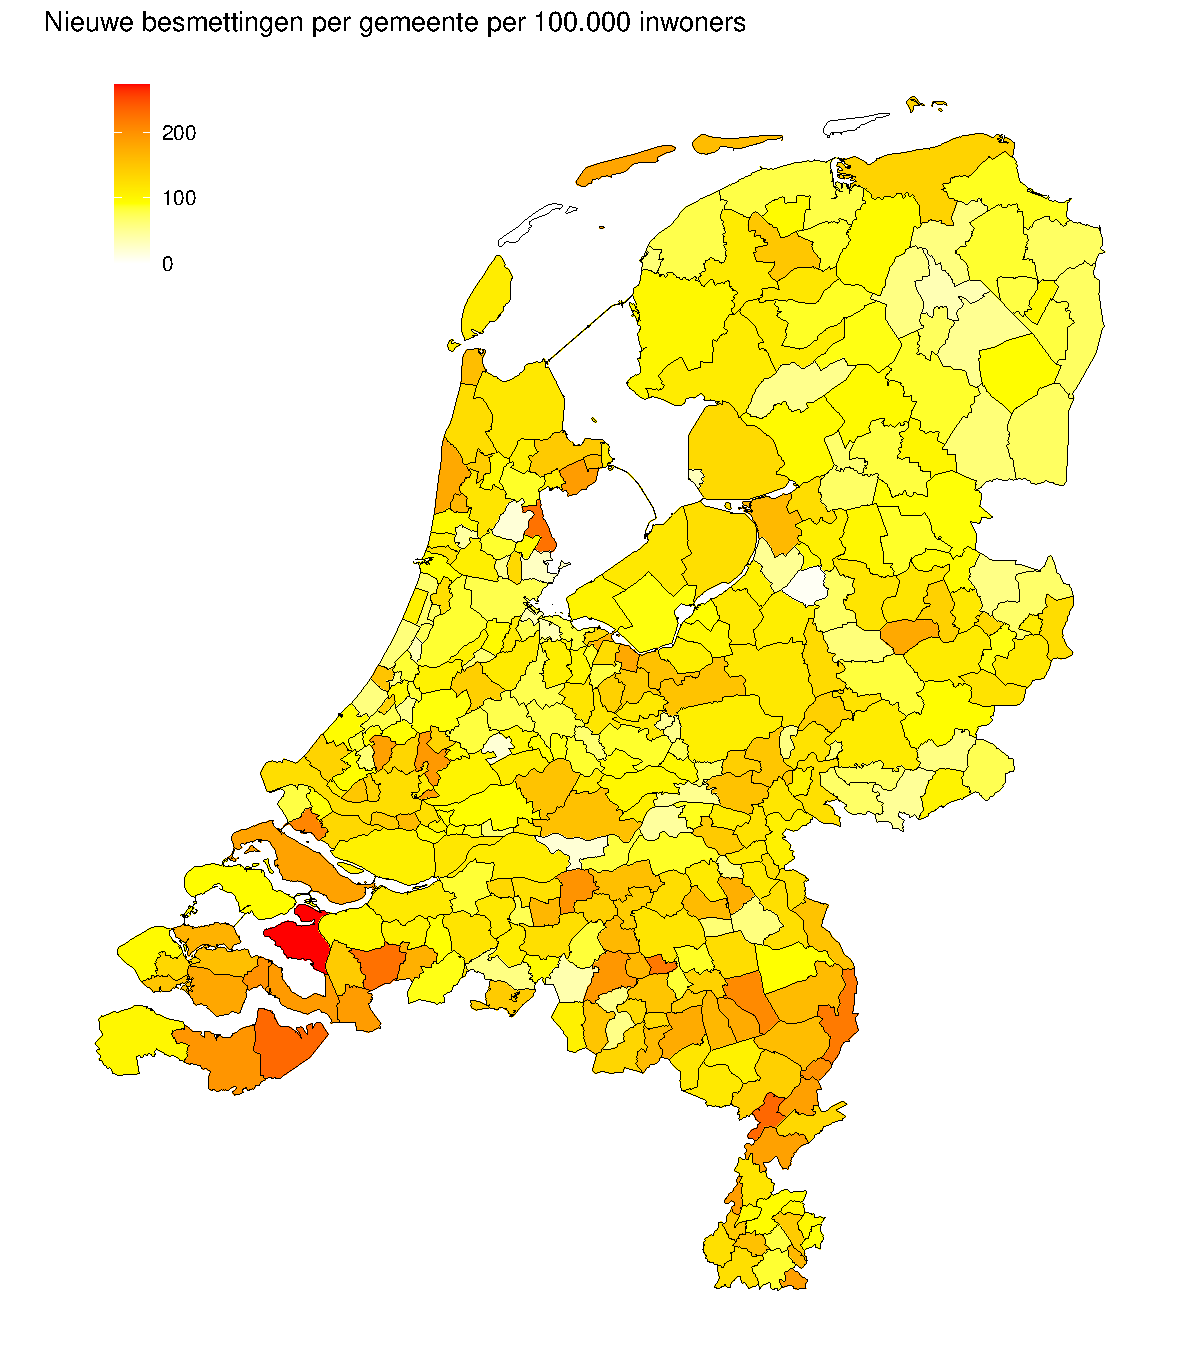
\includegraphics{daily_report_files/figure-latex/Gemeentes - sinds gisteren-1.pdf}
\caption{(\#Gemeentes - sinds gisteren) Aantal, sinds gisteren, bij de GGD'en gemelde COVID-19 patiënten per 100.000 inwoners per gemeente}
\end{figure}

\newpage

\hypertarget{kaart-met-covid-19-meldingen-per-gemeente-in-de-afgelopen-week}{%
\section{Kaart met COVID-19 meldingen per gemeente in de afgelopen week}\label{kaart-met-covid-19-meldingen-per-gemeente-in-de-afgelopen-week}}

\begin{figure}
\centering
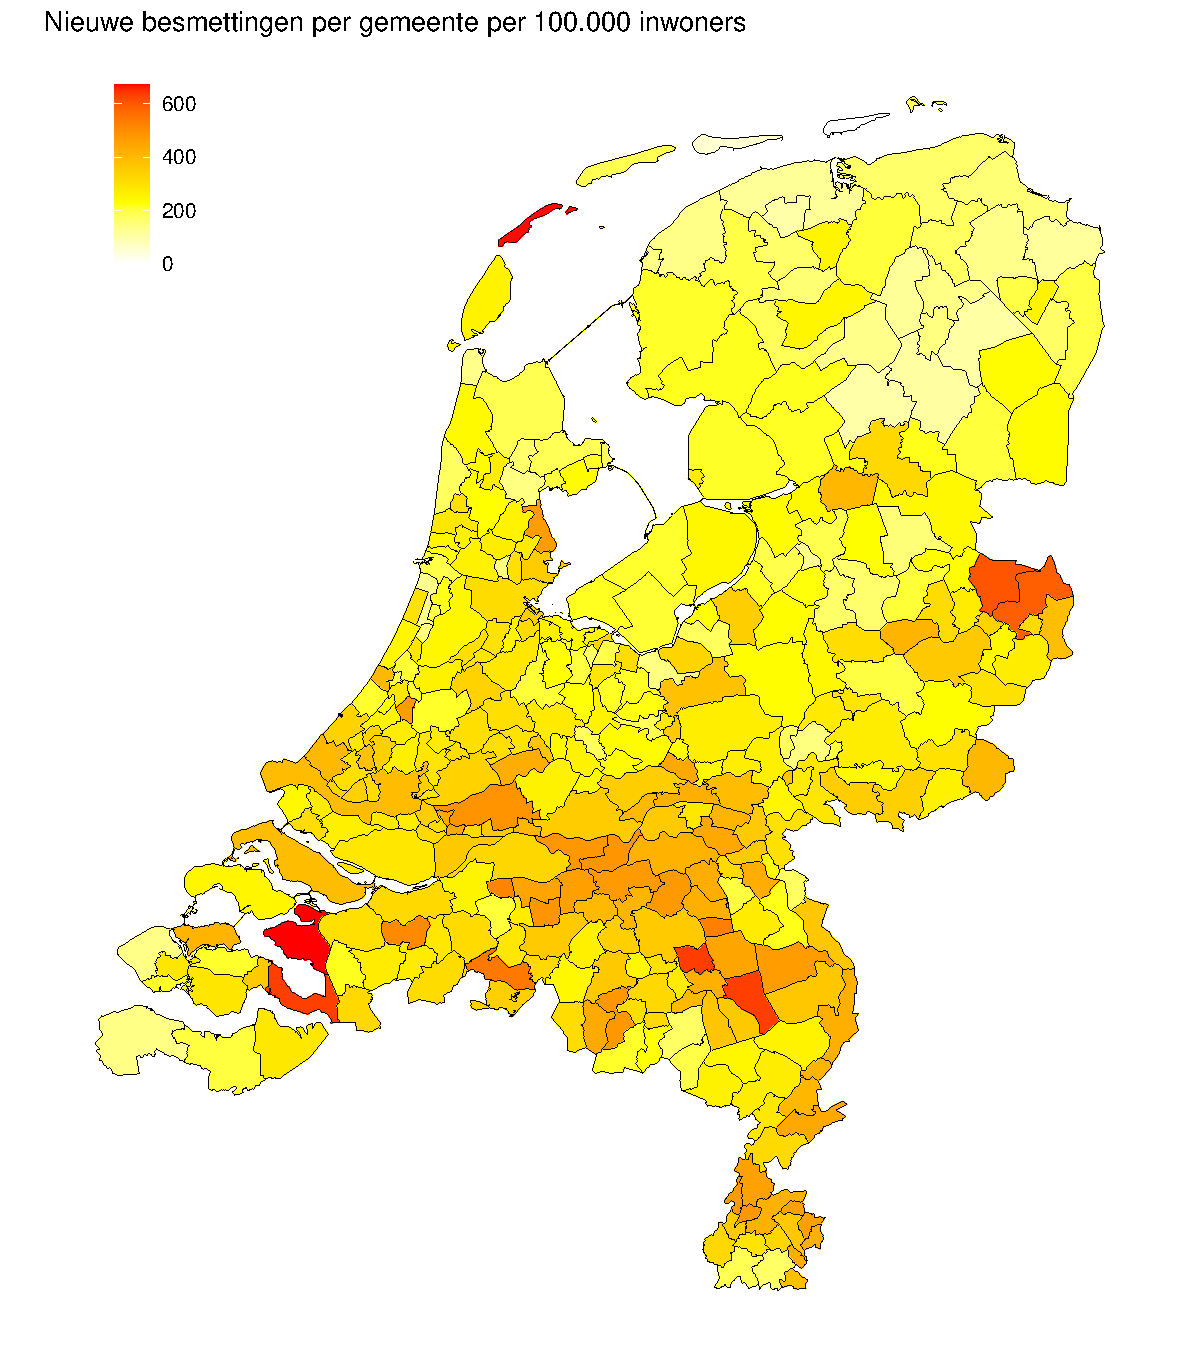
\includegraphics{daily_report_files/figure-latex/Gemeentes - Sinds vorige week-1.pdf}
\caption{(\#Gemeentes - Sinds vorige week) Aantal in de afgelopen week bij de GGD'en gemelde COVID-19 patiënten per 100.000 inwoners per gemeente.}
\end{figure}

\newpage

\hypertarget{aantal-covid-19-meldingen-per-provincie-in-de-afgelopen-twee-weken}{%
\section{Aantal COVID-19 meldingen per provincie in de afgelopen twee weken}\label{aantal-covid-19-meldingen-per-provincie-in-de-afgelopen-twee-weken}}

\begin{table}
\centering
\begin{threeparttable}
\begin{tabular}{lrrrrrr}
\toprule
\multicolumn{1}{c}{ } & \multicolumn{2}{c}{Besmettingen} & \multicolumn{2}{c}{Ziekenhuisopnames} & \multicolumn{2}{c}{Overleden} \\
\cmidrule(l{3pt}r{3pt}){2-3} \cmidrule(l{3pt}r{3pt}){4-5} \cmidrule(l{3pt}r{3pt}){6-7}
Provincie & Totaal & /100000 & Totaal & /100000 & Totaal & /100000\\
\midrule
Drenthe & 1901 & 382.4 & 15 & 3.0 & 7 & 1.4\\
Flevoland & 2270 & 524.4 & 17 & 3.9 & 8 & 1.8\\
Fryslân & 3312 & 506.6 & 18 & 2.8 & 6 & 0.9\\
Gelderland & 13406 & 636.6 & 76 & 3.6 & 32 & 1.5\\
Groningen & 1695 & 288.5 & 6 & 1.0 & 3 & 0.5\\
Limburg & 9053 & 810.1 & 64 & 5.7 & 34 & 3.0\\
Noord-Brabant & 12612 & 487.8 & 52 & 2.0 & 18 & 0.7\\
Noord-Holland & 12000 & 414.5 & 75 & 2.6 & 13 & 0.4\\
Overijssel & 6933 & 593.1 & 35 & 3.0 & 15 & 1.3\\
Utrecht & 7163 & 524.6 & 32 & 2.3 & 10 & 0.7\\
Zeeland & 2339 & 605.3 & 22 & 5.7 & 3 & 0.8\\
Zuid-Holland & 19829 & 530.3 & 131 & 3.5 & 29 & 0.8\\
\bottomrule
\end{tabular}
\begin{tablenotes}
\item \textit{Note: } 
\item Aantal bij de GGD’en gemelde COVID-19 patiënten, in het ziekenhuis opgenomen COVID-19 patiënten en overleden COVID-19 patiënten per provincie van 19 oktober t/m 02 november 10:00 uur, totaal en per 100.000 inwoners
\end{tablenotes}
\end{threeparttable}
\end{table}

\newpage

\hypertarget{aantal-covid-19-meldingen-per-ggd-in-de-afgelopen-twee-weken}{%
\section{Aantal COVID-19 meldingen per GGD in de afgelopen twee weken}\label{aantal-covid-19-meldingen-per-ggd-in-de-afgelopen-twee-weken}}

\begin{table}
\centering\begingroup\fontsize{10}{12}\selectfont

\begin{threeparttable}
\begin{tabular}{lrrrrrr}
\toprule
\multicolumn{1}{c}{ } & \multicolumn{2}{c}{Besmettingen} & \multicolumn{2}{c}{Ziekenhuisopnames} & \multicolumn{2}{c}{Overleden} \\
\cmidrule(l{3pt}r{3pt}){2-3} \cmidrule(l{3pt}r{3pt}){4-5} \cmidrule(l{3pt}r{3pt}){6-7}
GGD & Totaal & /100000 & Totaal & /100000 & Totaal & /100000\\
\midrule
Dienst Gezondheid \& Jeugd ZHZ & 3683 & 795.3 & 13 & 2.8 & 2 & 0.4\\
GGD Amsterdam & 4754 & 440.7 & 39 & 3.6 & 8 & 0.7\\
GGD Brabant-Zuidoost & 3261 & 413.2 & 7 & 0.9 & 5 & 0.6\\
GGD Drenthe & 1905 & 383.0 & 15 & 3.0 & 7 & 1.4\\
GGD Flevoland & 2267 & 523.0 & 17 & 3.9 & 8 & 1.8\\
GGD Fryslân & 3327 & 508.8 & 18 & 2.8 & 6 & 0.9\\
GGD Gelderland-Zuid & 3596 & 633.2 & 26 & 4.6 & 10 & 1.8\\
GGD Gooi en Vechtstreek & 1199 & 460.1 & 5 & 1.9 & 1 & 0.4\\
GGD Groningen & 1637 & 277.5 & 6 & 1.0 & 2 & 0.3\\
GGD Haaglanden & 4801 & 424.7 & 43 & 3.8 & 12 & 1.1\\
GGD Hart voor Brabant & 5578 & 513.6 & 20 & 1.8 & 5 & 0.5\\
GGD Hollands-Midden & 5433 & 662.8 & 30 & 3.7 & 7 & 0.9\\
GGD Hollands-Noorden & 2322 & 346.9 & 15 & 2.2 & 3 & 0.4\\
GGD IJsselland & 3918 & 729.0 & 19 & 3.5 & 9 & 1.7\\
GGD Kennemerland & 2281 & 412.4 & 11 & 2.0 & 1 & 0.2\\
GGD Limburg-Noord & 4724 & 901.2 & 29 & 5.5 & 15 & 2.9\\
GGD Noord- en Oost-Gelderland & 4976 & 596.2 & 20 & 2.4 & 11 & 1.3\\
GGD Regio Utrecht & 7162 & 1130.8 & 32 & 5.1 & 11 & 1.7\\
GGD Rotterdam-Rijnmond & 5890 & 430.7 & 45 & 3.3 & 8 & 0.6\\
GGD Twente & 3023 & 226.6 & 16 & 1.2 & 6 & 0.4\\
GGD West-Brabant & 3771 & 527.9 & 25 & 3.5 & 8 & 1.1\\
GGD Zaanstreek/Waterland & 1484 & 436.1 & 5 & 1.5 & 0 & 0.0\\
GGD Zeeland & 2338 & 604.5 & 22 & 5.7 & 3 & 0.8\\
GGD Zuid-Limburg & 4342 & 730.4 & 35 & 5.9 & 20 & 3.4\\
Veiligheids- en Gezondheidsregio Gelderland-Midden & 4841 & 685.7 & 30 & 4.2 & 10 & 1.4\\
\bottomrule
\end{tabular}
\begin{tablenotes}
\item \textit{Note: } 
\item Aantal bij de GGD’en gemelde COVID-19 patiënten, in het ziekenhuis opgenomen COVID-19 patiënten en overleden COVID-19 patiënten per GGD van 19 oktober t/m 02 november 10:00 uur, totaal en per 100.000 inwoners
\end{tablenotes}
\end{threeparttable}
\endgroup{}
\end{table}

\newpage

\hypertarget{ziekenhuisopnames-nice-in-de-afgelopen-twee-weken}{%
\section{Ziekenhuisopnames (NICE) in de afgelopen twee weken}\label{ziekenhuisopnames-nice-in-de-afgelopen-twee-weken}}

\begin{table}
\centering\begingroup\fontsize{10}{12}\selectfont

\begin{threeparttable}
\begin{tabular}{lrrrrrr}
\toprule
\multicolumn{1}{c}{ } & \multicolumn{2}{c}{Aanwezig} & \multicolumn{2}{c}{Opnames} & \multicolumn{2}{c}{Overleden} \\
\cmidrule(l{3pt}r{3pt}){2-3} \cmidrule(l{3pt}r{3pt}){4-5} \cmidrule(l{3pt}r{3pt}){6-7}
Leeftijd & Kliniek & IC & Kliniek & IC & Kliniek & IC\\
\midrule
<20 & 44 & 0 & 66 & 1 & 0 & 0\\
20 - 24 & 6 & 0 & 22 & 0 & 0 & 0\\
25 - 29 & 15 & 5 & 24 & 6 & 0 & 1\\
30 - 34 & 10 & 6 & 38 & 6 & 0 & 0\\
35 - 39 & 17 & 7 & 32 & 12 & 0 & 1\\
40 - 44 & 33 & 13 & 50 & 12 & 0 & 0\\
45 - 49 & 28 & 11 & 54 & 16 & 0 & 0\\
50 - 54 & 44 & 25 & 58 & 22 & 0 & 3\\
55 - 59 & 41 & 27 & 76 & 28 & 4 & 0\\
60 - 64 & 70 & 33 & 107 & 42 & 4 & 11\\
65 - 69 & 90 & 44 & 125 & 45 & 5 & 10\\
70 - 74 & 124 & 44 & 149 & 42 & 12 & 12\\
75 - 79 & 177 & 20 & 229 & 26 & 16 & 8\\
80 - 84 & 158 & 2 & 206 & 8 & 34 & 5\\
85 - 89 & 117 & 0 & 148 & 1 & 34 & 0\\
>90 & 57 & 0 & 86 & 0 & 19 & 0\\
\bottomrule
\end{tabular}
\begin{tablenotes}
\item \textit{Note: } 
\item Aantal bij NICE gemelde COVID-19 patiënten: in het ziekenhuis aanwezige COVID-19 patiënten, opnames, en overleden COVID-19 patiënten in het ziekenhuis van 19 oktober t/m 02 november 15:15 uur
\end{tablenotes}
\end{threeparttable}
\endgroup{}
\end{table}

\newpage

\hypertarget{leeftijdsverdeling-en-man-vrouwverdeling-van-covid-19-patiuxebnten-in-de-afgelopen-twee-weken}{%
\section{Leeftijdsverdeling en man-vrouwverdeling van COVID-19 patiënten in de afgelopen twee weken}\label{leeftijdsverdeling-en-man-vrouwverdeling-van-covid-19-patiuxebnten-in-de-afgelopen-twee-weken}}

\begin{table}
\centering\begingroup\fontsize{11}{13}\selectfont

\begin{threeparttable}
\begin{tabular}{lrrrrrr}
\toprule
\multicolumn{1}{c}{ } & \multicolumn{2}{c}{Besmettingen} & \multicolumn{2}{c}{Ziekenhuisopnames} & \multicolumn{2}{c}{Overleden} \\
\cmidrule(l{3pt}r{3pt}){2-3} \cmidrule(l{3pt}r{3pt}){4-5} \cmidrule(l{3pt}r{3pt}){6-7}
Leeftijdsgroep & Totaal & \% & Totaal & \% & Totaal & \%\\
\midrule
<50 & 2 & 0.0 & 1 & 0.2 & 2 & 1.1\\
0-9 & 6961 & 7.5 & 14 & 2.6 & NA & NA\\
10-19 & 12009 & 13.0 & 2 & 0.4 & NA & NA\\
20-29 & 14300 & 15.5 & 6 & 1.1 & NA & NA\\
30-39 & 14360 & 15.5 & 30 & 5.5 & NA & NA\\
40-49 & 12771 & 13.8 & 38 & 7.0 & NA & NA\\
50-59 & 11847 & 12.8 & 53 & 9.8 & 4 & 2.2\\
60-69 & 9395 & 10.2 & 111 & 20.4 & 13 & 7.3\\
70-79 & 6643 & 7.2 & 127 & 23.4 & 34 & 19.1\\
80-89 & 3341 & 3.6 & 137 & 25.2 & 83 & 46.6\\
90+ & 884 & 1.0 & 24 & 4.4 & 42 & 23.6\\
\bottomrule
\end{tabular}
\begin{tablenotes}
\item[1] Leeftijdsverdeling van bij de GGD’en gemelde COVID-19 patiënten, in het ziekenhuis opgenomen COVID-19 patiënten en overleden COVID-19 patiënten van 19 oktober t/m 02 november 10:00 uur.
\item[2] Overlijdensgevallen van patiënten jonger dan 50 jaar oud worden door het RIVM in de casusdata gegroepeerd in de categorie <50. Deze overlijdensgevallen zijn hier dus niet zichtbaar in deze leeftijdsgroepen maar alleen via de groep '<50'.
\end{tablenotes}
\end{threeparttable}
\endgroup{}
\end{table}

\newpage

\begin{table}
\centering\begingroup\fontsize{11}{13}\selectfont

\begin{threeparttable}
\begin{tabular}{lrrrrrr}
\toprule
\multicolumn{1}{c}{ } & \multicolumn{2}{c}{Besmettingen} & \multicolumn{2}{c}{Ziekenhuisopnames} & \multicolumn{2}{c}{Overleden} \\
\cmidrule(l{3pt}r{3pt}){2-3} \cmidrule(l{3pt}r{3pt}){4-5} \cmidrule(l{3pt}r{3pt}){6-7}
Geslacht & Totaal & \% & Totaal & \% & Totaal & \%\\
\midrule
Vrouw & 48616 & 52.6 & 233 & 42.9 & 77 & 43.3\\
Man & 43897 & 47.4 & 310 & 57.1 & 101 & 56.7\\
Onbekend & 0 & 0.0 & 0 & 0.0 & NA & NA\\
\bottomrule
\end{tabular}
\begin{tablenotes}
\item \textit{Note: } 
\item Man-vrouwverdeling van bij de GGD’en gemelde COVID-19 patiënten, in het ziekenhuis opgenomen COVID-19 patiënten en overleden COVID-19 patiënten van 19 oktober t/m 02 november 10:00 uur.
\end{tablenotes}
\end{threeparttable}
\endgroup{}
\end{table}
\newpage


\end{document}
